\documentclass{report}

% The ams packages are required to insert any mathematical symbols that you may require
\usepackage{amsfonts}
\usepackage{amssymb}
\usepackage{amsmath}
\usepackage{amsthm}
% This package is used for embedding things like PDFs and JPEGs into your document
\usepackage{graphicx}
% This package is used for drawing pictures (such as trees)
\usepackage{tikz}
\usetikzlibrary{arrows,automata}
% These packages are used for adding pseudo-code to your document
\usepackage{algorithm2e}
\usepackage{algorithmic}
% This package is for if you require an appendix
\usepackage{appendix}

\usepackage{datetime}
\usepackage{fancyhdr}
\usepackage{semantic}
\usepackage[noload]{qtree}
\usepackage{comment}
\usepackage{pdflscape}
\usepackage{graphicx}
\usepackage[margin=1in]{geometry}
\usepackage{moreverb}
\usepackage{caption}
\usepackage{url}
\usepackage{layout}

\usepackage[annatar]{tengwarscript}

\usetikzlibrary{shapes}
\usetikzlibrary{arrows}

\newcommand{\pr}{\mathbb{P}}
\newcommand{\tengt}{\mbox{\Ttinco}}

\DeclareMathOperator*{\argmax}{arg\,max}
\DeclareMathOperator*{\argmin}{arg\,min}

\begin{document}

\begin{titlepage}
\title{An Investigation of Stochastic Processes on Human-Generated Data}
\author{Tim Jones}
%\maketitle

\centering{\textsc{\huge{An Investigation into Stochastic Processes for Modelling Human-Generated Data}}}\\[1.5cm]

\centering{\textsc{\large{A 20-cp 3rd year project}}}\\[1.5cm]

\begin{minipage}{0.4\textwidth}
\begin{flushleft} \large
\emph{Author:}\\
Tim Jones
\end{flushleft}
\end{minipage}
\begin{minipage}{0.4\textwidth}
\begin{flushright} \large
\emph{Supervisor:} \\
Dr. Gordon Ross
\end{flushright}
\end{minipage}\\[1.5cm]

\vfill

Rendered on \today

\end{titlepage}

\tableofcontents

\chapter{Introduction}

Modelling human-generated ``random" data is notoriously difficult. Human event data arises in a variety of real-world situations, for example when inspecting network traffic or email communications. Being able to spot anomalies has important applications in botnet detection and spotting suspicious behaviour on social networks. In this project, we attempted to model the behaviour of one user of twitter using various random processes. Ideally, we would find a good model for twitter in general, but one user makes a worthy starting point, and twitter provides an easily accessible representation of such data without trawling through net logs or other people's email accounts. The user was observed over the course of around 6 months posting (emitting) a little over 3,300 tweets. The goal is to find some kind of model to fit these data, without using a hideously large number of parameters.

The data are visualised in Figure \ref{raw_data}. We see a little seasonality - the user seems to be going to sleep at some time, waking up at another time, as well as some ``burstiness", the user will produce a very rapid series of tweets in a very short time. Being able to detect these things would let us intuitively decide whether a fit is good or not, but principally we'll be reliant on statistical tests to judge how good our model is.

Chapter \ref{zoo} will define a series of stochastic processes which will we can use for modelling the data, and then chapter \ref{techniques} will apply the more relevant ones. Of particular note is the Markov-Modulated Poisson Process defined in \textsection\ref{mmppdef}, which several authors \cite{mmpp1}\cite{mmpp2}\cite{mmpp3} have postulated will provide a good model due to its doubly-stochastic nature -- the intuition being that the tweets are a stochastic process, and the parameters of that stochastic process themselves follow another stochastic process. Appendix \ref{fun} also describes a subsidiary result which was spotted during this project, and which may have rather useful applications in other fields.

\begin{figure}[h]
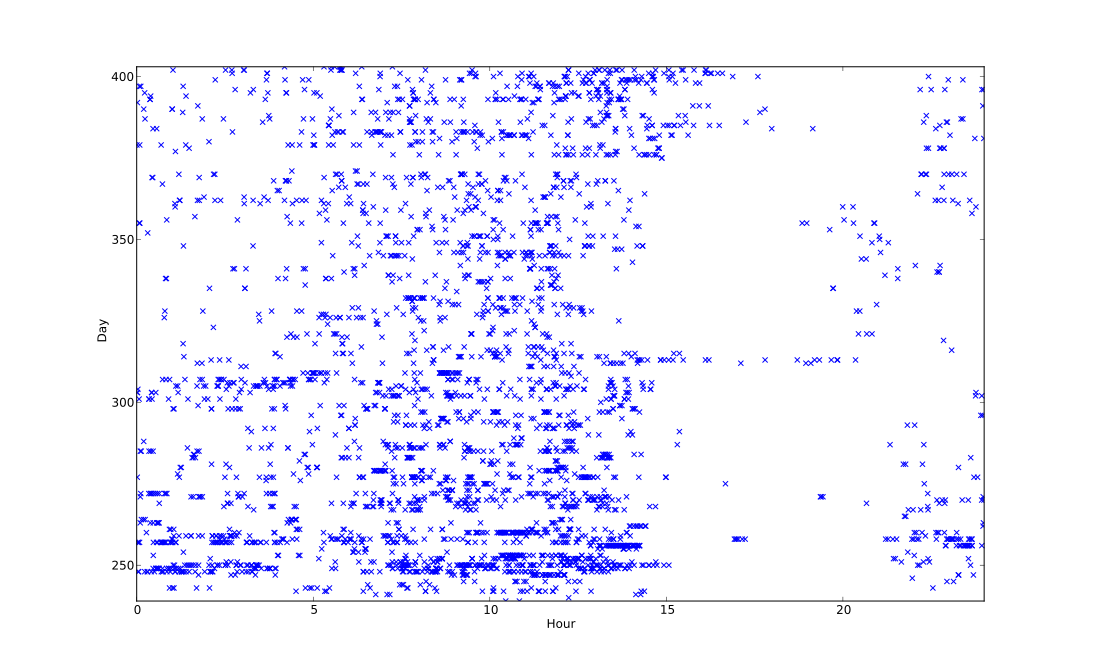
\includegraphics[width = 0.5\textwidth]{./images/raw_data.png}
\caption{The raw data gathered from the twitter user. Each blue cross marks a tweet at a particular time. The 24 hours of a day run across the x axis, and the days within our 6 months run up the y-axis, so a point at $(17.5, 256)$ is a tweet at 5:30pm 256 days into the observation.}
\label{raw_data}
\end{figure}

\chapter{A Zoo of Stochastic Processes}

\section{Markov Chains}

\subsection{A Formal Definition}

A stochastic process \cite[p590]{doob96} is a collection $\{X_t  | t \in T\}$ (sometimes $X(t)$ for continuous $T$) of random variables. These collections may be indexed arbitrarily, but tend to be used to describe the evolution of some random series of events, using $T$ to be some representation of either discrete or continuous time, for instance $X_t$ may be the number of observed emissions from a radioactive source after $t$ minutes or the licence plate of the $t^{th}$ car to go past a speed camera.

A Discrete Time Markov Chain (DTMC) is a particular form of discrete-time stochastic process - one which obeys the Markov Property. We usually set $T=\{0,1,2,...\}=\mathbb{N}$ and we say that $(X_t)_{t \in \mathbb{N}}$ obeys the Markov Property iff

$$
\forall t \in T, s \in S \quad \pr (X_{t+1} = s | X_0, X_1, ... X_t) = \pr (X_{t+1} = s | X_t)\cite{mwmarkov}
$$

We refer to $S$ as the state-space, each $s \in S$ is a state, and $X_t$ represents the state at time t. We usually write the Markov Property as ``given the present, the future is conditionally independent of the past" \cite{mwmarkov}.
%COVER THIS IN G&S CITATIONS

There is also a Continuous Time Markov Chain (CTMC, sometimes CTMP for Continuous Time Markov Process). We set $T=\mathbb{R}^{+}$,and define a similar Markov Property;

$$
\forall \delta > 0, s \in S \quad \pr (X(t+\delta) = s | \{X(\tau), \tau < t\}) = \pr (X(t+\delta) = s | X_t)
$$

We'll be dealing exclusively with the discrete-space case in this project, ie a Markov Chain where $S$ is discrete, though we'll need to use both continuous and discrete times. It is popular for many authors to set $S \subseteq \mathbb{Z}$, though our states can be integers, real numbers, popes, or any other completely arbitrary non-empty set. Where $S$ and $T$ are discrete, we define $\mathbf{\delta} = (\delta_i)_{i \in S}$, the initial probability vector, and $\Pi = (\pi_{ij})_{(i,j) \in S^2}$, the matrix of transition probabilities, such that,

\begin{align*}
\delta_i &= \pr (X_0 = i) \\
\pi_{ij} &= \pr(X_{t+1} = j | X_t = i) \forall t \in \mathbb{N}
\end{align*}

Note that, from the Markov Property, we have that $\Pi$ does not depend on time. We refer to this independence as homogeneity. Every DTMC can be uniquley defined by the triple $(S,\delta,\Pi)$. Naturally, the row sums of $\Pi$ should be $1$, ie

$$
\forall i \in S, \; \sum_{j \in S} \pi_{ij} = 1
$$

For CTMCs, rather than a transition probability matrix, a transition rate matrix $Q$ is defined as;

$$
\forall i,j \in S, \delta>0 \quad \pr (X(t+\delta)=j|X(t)=i) = q_{ij}\delta + o(\delta)
$$

Where $o(\delta)$ is some function such that $o(\delta) -> 0$ as $\delta -> 0$. This gives us that

$$
\forall i,j \in S, \delta>0 \quad \pr (X(t+\delta)=j|X(t)=i) = (e^{\delta Q})_{ij}
$$

That is, the $i,j^{th}$ element of the matrix exponential of $\delta Q$. With the initial probability vector $\delta$ defined as before, we can uniquely define any CTMP with the triple $(S,\delta,Q)$. $Q$'s row sums are always 0, with all off-diagonal elements being positive, and all diagonal elements being negative, ie

\begin{align*}
\forall i,j \in S, i \neq j => q_{ij} > 0 \\
\forall i \in S, q_{ii} = -\sum_{j \neq i} q_{ij}
\end{align*}

\subsection{An Intuitive Interpretation}

Whilst the above defines Markovian Processes, it fails to describe them in any intuitive way. Before attempting to use them, it is important to be able to deal with both the continuous and discrete-time Markov Chains in an intuitive way. My personal preferred method is to use edge-weighted directed graphs \cite{mwgraph}. Each state in $S$ is given a node in the graph, and for each $i,j \in S$ the edge $(i,j)$ is given weight $\pi_{ij}$ in the discrete case and $q_{ij}$ in the continuous case.

As an example, let's use the following definitions, with $\delta$ and $\Pi$ indexed in the order the elements of $S$ are written;

\begin{align*}
S &= \{\mbox{John Paul II}, \mbox{Adrian I}\}\\
\delta &= \left(1,0\right)\\
\Pi &=
\bordermatrix{      & JP2&A1 \cr
                JP2 & 0.3 &  0.7 \cr
                A1  & 0.9 &  0.1 
			}
\end{align*}

This defines a Discrete Time Markov Chain with the following graph:

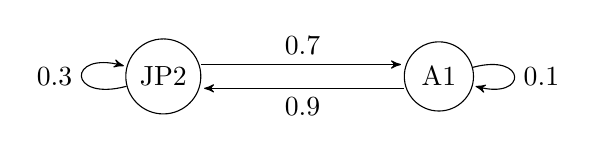
\begin{tikzpicture}[->,>=stealth',shorten >=1pt,auto,node distance=3.5cm]
  \node[state]         (r)                     {JP2};
  \node[state]         (b)  [right of = r]     {A1};

  \path  (r) edge[loop left]   node {$0.3$} (r)
         ([yshift=1ex]r.east) edge node {$0.7$} ([yshift=1ex]b.west)

         (b) edge[loop right]   node {$0.1$} (b)
         ([yshift=-1ex]b.west)edge node {$0.9$} ([yshift=-1ex]r.east)

  ;
\end{tikzpicture}


We can then say that a DTMC will hop from node to node at each time step with probabilities defined by the weights of the edges between the current node and its neighbors, and can be simulated by algorithm \ref{algmc}.

\begin{algorithm}
\SetAlgoLined
\SetKwInOut{Input}{input}
\SetKwInOut{Output}{output}

\caption{A Simulation Algorithm for the generic Markov Chain}\label{algmc}
\Input{$(S,\delta,\Pi)$, a Markov Chain, and $T$, a maximum number of steps to simulate}
\Output{$\mathbf{s}$, a vector of states $s_i$, recording the sequence of states visited by the chain}

\Begin{
	$s_1 <- \sigma \quad wp \; \; \delta_\sigma$ \tcc{s0 takes on state sigma 
											with probability delta sigma}
	\For{$n <- 2$ \KwTo $T$}{
		$s_n <- \sigma \quad wp \; \; \pi_{s_{n-1},\sigma}$
		\tcc{sn takes on state sigma with the relevant probability}
	}
	\KwRet $\mathbf{s}$
}
\end{algorithm}

A CTMP is slightly more complex; on arriving in a state $i$, a random time $T \sim Exp(-q_{ii})$ is generated. The CTMP will remain in state $i$ for $T$ units of time, then jump to state $j$ with probability $\frac{-q_{ij}}{q_{ii}}$. We can simulate a CTMP with algorithm \ref{algctmp}.

\begin{algorithm}
\SetAlgoLined
\SetKwInOut{Input}{input}
\SetKwInOut{Output}{output}

\caption{A Simulation Algorithm for the generic CTMP}\label{algctmp}
\Input{$(S,\delta,Q)$, a CTMP, and $T$, a maximum time for which to simulate the process}
\Output{$\mathbf{t}$, a vector of pairs $(t_i,s_i)$, recording the time and destination of the $i^{th}$ transition.}

\Begin{
	$t_0 <- 0$ \\
	$s_0 <- \sigma \quad wp \; \; \delta_\sigma$ \tcc{s0 takes on state sigma 
											with probability delta sigma}
	$n <- 0$\\
	\While{$t_n<T$}{
		$n <- n+1$\\
		$\tau <- Exp(-q_{ii})$ \tcc{tau takes on an exponentially distributed 
									random value}
		$t_n <- t_{n-1} + \tau$\\
		$s_n <- \sigma \quad wp \; \; \frac{-q_{i\sigma}}{q_{ii}}$
		\tcc{sn takes on state sigma with the given probability}
	}
	\KwRet $((t_0,s_0),...,(t_{n-1},s_{n-1}))$
}
\end{algorithm}

\subsection{The Poisson Process}

The simplest form of CTMP is the homogeneous Poisson rocess, where $S = \mathbb{N}$ and $\forall i \in S, q_{ii}=-\lambda, q_{i,i+1} = \lambda$. We call $\lambda$ the rate of this process. If $N(t)$ is a Poisson process, we then have that

$$
\forall i \in \mathbb{N}, t,\varepsilon \in \mathbb{R}^{+}, \pr (N(t+\varepsilon) = i+1 | N(t) = i) = \lambda \varepsilon + o(\varepsilon)
$$

Note that $N$ is the associating counting process - a stochastic process - not a distribution or a random variable. The graph for this process is similarly simple

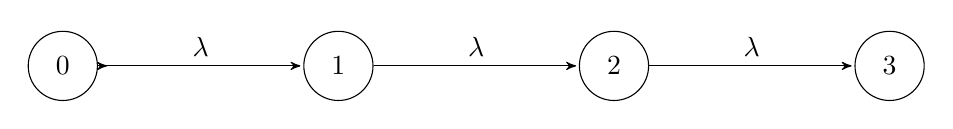
\begin{tikzpicture}[->,>=stealth',shorten >=1pt,auto,node distance=3.5cm]
  \node[state]         (0)                     {0};
  \node[state]         (1)  [right of = 0]     {1};
  \node[state]         (2)  [right of = 1]     {2};
  \node[state]         (3)  [right of = 2]     {3};

  \path  (0) edge   node {$\lambda$} (1)
         (1) edge   node {$\lambda$} (2)
         (2) edge   node {$\lambda$} (3)
  ;
  \draw  (0.east) -- ([xshift=1ex]0.east);
\end{tikzpicture}

Implicit from this, we see that the process can only increase - once leaving a state, we never return, so we can define the emission times $t_n$, as $t_n = \min\{t | N(t)\geqslant n\}$. We can also define $\tau_n = t_n-t_{n-1}$, the inter-arrival times for the $n^{th}$ jump for $n \{1,2,...\}$. We refer to these as emissions and arrivals since a Poisson Process generally models a counting process whereby we record the times at which we observe things happening, eg the times at which radioactive particles are detected from a radioactive material. The most crucial property of the Poisson process for this work, implicit from the simulation algorithm above, is that

$$
\forall n \in \mathbb{N} \; \; \tau_n \sim Exp(\lambda)
$$

That is, the inter-arrival times are all exponentially distributed. A modification of the generic CTMP simulation algorithm can be made for simulating  a Poisson Process. Since it's only possible to jump from state $i$ to state $i+1$, we need not record the destinations of each jump; jump $i$ will always take us to state $i$. This is detailed in algorithm \ref{algpp}.

\begin{algorithm}
\SetAlgoLined
\SetKwInOut{Input}{input}
\SetKwInOut{Output}{output}

\caption{A Simulation Algorithm for the Poisson Process}\label{algpp}
\Input{$\lambda$, a poisson process rate and $T$, a maximum time for which to simulate}
\Output{$\mathbf{t}$, the emission times of a Poisson process of rate $\lambda$ terminating before time $T$}

\Begin{
	$t_0 <- 0$\\
	$n <- 0$\\
	\While{$t_n<T$}{
		$n <- n+1$\\
		$\tau <- Exp(\lambda)$ \tcc{tau takes on an exponentially distributed 
									random value}
		$t_n <- t_{n-1} + \tau$
	}
	\KwRet $(t_0,...,t_{n-1})$
}
\end{algorithm}

We can also sacrifice the Markov Property to define an inhomogeneous Poisson process. Everything remains from before, except rather than having a rate parameter $\lambda \in \mathbb{R}^{+}$, we have a rate function $\lambda : \mathbb{R}^{+} -> \mathbb{R}^{+}$, where

$$
\forall i \in \mathbb{N}, t,\delta \in \mathbb{R}^{+}, \pr (N(t+\delta) = i+1 | N(t) = i) = \lambda(t) \delta + o(\delta)
$$

Since this process is no longer Markovian, it makes little sense to draw its transition rate graph, however it remains a powerful tool. Simulating one of these is, however, less simple. The algorithm for doing so is based on Bernoulli thinning %cite
and is equivalent to algorithm \ref{algthin}

\begin{algorithm}
\SetAlgoLined
\SetKwInOut{Input}{input}
\SetKwInOut{Output}{output}

\caption{A Thinning Algorithm for Poisson Processes}\label{algthin}
\Input{$\lambda : [0,T] -> [0,\lambda_{max}]$, a desired rate function for the resulting Poisson Process, and $\mathbf{t}$, the emission times of a Poisson Process of rate no greater than $\lambda_{max}$, terminating before time $T$, indexed from 1 to $n$}
\Output{$\mathbf{t'}$, the emission times an inhomogeneous Poisson Process with rate function $\lambda$}

\Begin{
	$j <- 0$
	\For{$i <- 1$ \KwTo $n$}{
		$r <- U(0,1)$ \tcc{r takes on a uniformly distributed random value in 	
							[0,1]}
		\If{$r < \frac{\lambda(t_i)}{\lambda_{max}}$}{
			$t'_j <- t_i$ \\
			$j <- j+1$
		}
	}
	\KwRet $\mathbf{t'}$
}
\end{algorithm}

So we keep each point in the given poisson process with a probability proportional to the rate function. If we can find an upper bound for our rate function, we can combine algorithms \ref{algpp} and \ref{algthin} to simulate arbitrary inhomogeneous poisson processes.

\section{Hidden Markov Models}

The Hidden Markov Model is an extention of the Markov Chain.

With discrete time and state space, rather than having a directly observable Markov Chain, it is assumed that the process has an underlying unobservable Markov Chain. An observation space, $Y$ is defined, and a set of probability distrubtions, $\{p_s | s \in S\}$. Before jumping out of state $s$, the Markov Chain emits observation $y$ with probability $P_s(y)$. Alternatively, we can define a continuous $Y$ with probability densities instead of a probability distribution.

The traditional example is that of the ``unfair casino". Imagine the dealer at the casino has two six-sided dice. Die one is fair, but die two is weighted such that it never shows a 6, and shows the numbers 1 to 5 with equal probabilities. The dealer will clandestinely swap the dice with probability $0.1$ before rolling. He selects his first die uniformly. We can represent this as follows;

\begin{align*}
S &= \{1,2\}\\
\delta &= (0.5,0.5)\\
\Pi &= 
\left(
	\begin{matrix}
	0.9 & 0.1 \\
	0.1 & 0.9
	\end{matrix}
\right)\\
Y &= \{1,2,3,4,5,6\}\\
y \in Y => p_1(y) &= \frac{1}{6}\\
y \in Y \setminus \{6\} => p_2(y) &= \frac{1}{5}
\end{align*}

We can only observe the results of the dice rolls, but what we're interested in is the sequence of states entered by the model. Which die is the dealer using at which time?. Further to this, suppose we didn't know the above parameters in advance. We may also want to estimate them from our observations in some way.

\section{The Markov-Modulated Poisson Process}

The Markov-Modulated Poisson Process (MMPP) is a particular form of Hidden Markov Model. We assume that, underlying an emittor, there is a CTMP. Each state is tied to a fixed Poisson Process rate, so $S = \{\lambda_1,...,\lambda_n\}$. The instantaneous rate of the poisson process is then defined by the state in which the underlying CTMP resides. We can define such a process by letting $\mathbf{t} = ((t_0,s_0),...,(t_n,s_n))$ be a trace of the CTMP as generated by algorithm \label{algctmp}
, and $\lambda : [0,T]->S$ be the step function generated by simulating the underlying CTMP, ie;

$$
\lambda(\tau) = 
\begin{cases}
	s_i & \mbox{for} \quad \tau \in [t_i,t_{i+1}), \quad i \in [n-1]\\
	s_n & \mbox{for} \quad \tau \in [t_n,T]
\end{cases}
$$

We then have that an inhomogeneous poisson process of rate $\lambda$ is a single trace of this MMPP. In order to generate multiple traces, it is necessary for us to produce a new rate function $\lambda$ from the underlying CTMP for each trace.

Though this is correct, I personally find that it is simpler to imagine an MMPP as the concatenation of a series of poisson processes, each generated within a particular state of the underlying CTMP, eg the underlying CTMP enters state $s_1$ at time $t_1$. It generates emissions as a Poisson Process of rate $s_1$ for $t_2-t_1$ time units. It then stops acting like this poisson process, and starts generating emissions as a poisson process of rate $s_2$ for $t_3-t_2$ time units.

It's not immediately obvious that this intuition matches the definition, so it's worth arguing that this is the case.

Let $\lambda_1: [0,T_1) -> \mathbb{R}^{+}$ and $\lambda_2:[0,T_2) -> \mathbb{R}^{+}$ be two rate functions. Let $T = T_1 + T_2$, and define $\lambda$, the concatenation $\lambda = \lambda_1 || \lambda_2$, as;

$$
\lambda(\tau) = 
\begin{cases}
	\lambda_1(\tau) & \mbox{for} \quad \tau \in [0,T_1)\\
	\lambda_2(\tau-T_1) & \mbox{for} \quad \tau \in [T_1,T)
\end{cases}
$$

Let $\{N_1(t) | t \in [0,T1)\}$ be a poisson process of rate $\lambda_1$, similarly for $N_2$ and $N$, and let $\widetilde{N}$ be defined thus;

$$
\widetilde{N}(\tau) = 
\begin{cases}
	N_1(\tau) & \mbox{for} \quad \tau \in [0,T_1)\\
	N_1(T_1) + N_2(\tau-T_1) & \mbox{for} \quad \tau \in [T_1,T)
\end{cases}
$$

$\widetilde{N}$ represents my intuition that an MMPP can be formed by gluing together emissions from shorter fixed rate poisson processes, and $N$ represents the actual definition given above. If we can show that $\widetilde{N}$ and $N$ are ideentically distributed, then we can inductively apply this result to arbitrarily long concatenations, and hence to the generic MMPP.

Let $\tau \in [0,T_1)$ and $\varepsilon>0$ be such that $\tau + \varepsilon < T_1$. We then have that

\begin{align*}
\pr (\widetilde{N}(\tau+\varepsilon) - \widetilde{N}(\tau) = 1)
	&= \pr (N_1(\tau+\varepsilon) - N_1(\tau) = 1) \\
	&= \lambda_1(\tau)\varepsilon + o(\varepsilon) \\
	&= \lambda(\tau)\varepsilon + o(\varepsilon)
\end{align*} 

So $\widetilde{N}$ is similar to a poisson process of rate $\lambda$ within the range $[0,T_1)$.

Now let $\tau \in [T_1,T)$ and $\varepsilon>0$ be such that $\tau + \varepsilon < T$. We have that

\begin{align*}
\pr (\widetilde{N}(\tau+\varepsilon) - \widetilde{N}(\tau) = 1)
	&= \pr (N_2(\tau-T_1+\varepsilon) + N_1(T_1) - N_2(\tau-T_1) - N_1(T_1)= 1)\\
	&= \pr (N_2(\tau-T_1+\varepsilon) - N_2(\tau-T_1) = 1)\\
	&= \pr (N_2(\tau-T_1+\varepsilon) - N_2(\tau-T_1) = 1)\\
	&= \lambda_2(\tau-T_1)\varepsilon + o(\varepsilon) \\
	&= \lambda(\tau)\varepsilon + o(\varepsilon)
\end{align*}

So $\widetilde{N}$ is similar to a poisson process of rate $\lambda$ within the range $[T_1,T)$. We need not deal with the case where $\tau$ and $\tau+\varepsilon$ are either side of $T_1$, since we can always choose an $\varepsilon$ small enough such that this is not the case - these probabilities always assume that $\varepsilon$ is close to 0. So we have that $\widetilde{N}$ is distributed identically to $N$.

So concatenating two poisson processes of rates $\lambda_1$ and $\lambda_2$ produces a new poisson process of rate $\lambda_1||\lambda_2$, and it follows from simple induction that an MMPP can be thought of as the concatenation of multiple bounded-length homogeneous poisson processes of rates determined by the state of the underlying CTMP, and time bounds determined by the length of time spent in each state of the underlying CTMP.


\chapter{Potential Modelling Techniques}

Now that we've defined a selection of random processes, we can grab our data and start modelling it. We'll try out a few potential models, simulate some traces from them, and see how well we can re-establish the original model, then go on to discuss their use for this particular problem.

\section{Fitting a Non-Homogeneous Poisson Process}

The simplest place to start is with a non-homogeneous poisson process. We assume that the tweeter emits tweets according to an inhomogeneous poisson process, and attempt to find its rate function. For convenience, we'll describe our time in hours, though naturally the units could be arbitrary. We start by simulating a poisson process of known rate, and seeing how well we can recover the original rate function. We start with a simple step function,

$$
\lambda(t) = 
\begin{cases}
5  & \mbox{for} \quad 0  \leqslant t < 30\\
10 & \mbox{for} \quad 30 \leqslant t < 50\\
5  & \mbox{for} \quad 50 \leqslant t < 100
\end{cases}
$$

And we simulate the process for 100 hours, producing a trace such as;

%Put trace here

We can fit a step function by observing multiple traces of these poisson processes, taking the differences in emission times, then attempting to cluster them with the k-means algorithm%cite
. The average number of emissions per trace is the integral of the rate wrt time over the time interval for which we observe, ie if $N$ is the number of observed emissions in a single trace,

$$
\mathbb{E}(N) = \int^100_0 \lambda(t) \; dt = 600
$$

So if we run out 6 traces we'll observe roughly $3,600$ emissions, a little more than our real data set. Fitting a function to these gives us the results from %diagram

%Diagram here

Eyeballing this, we see that it's not a terrible fit in this first attempt, but if we try a more complex rate function, %diagram
happens

%Lots of steps in a step function

We could instead attempt to fit a polynomial function, but a smooth function is subject to one very large problem with twitter data - humans don't behave in a smooth manner. Our usage of twitter throughout a day does not vary along some continuum - in the simplest sense, we can't be half on and half off twitter at some given moment, but there's a worse problem, visible in %figure

% Trace of one day, showing bursts

We can see an important feature between 
%time1
and
%time2
. We'll call this a ``burst". The user is tweeting very rapidly for a short period of time. These bursts occur at random times throughout the day, and last for random lengths of time, but they all take on the same form. This heavily restricts our function. We can't simply say that at some particular time there is always a burst, but we also cannot deny their existence by smoothing them out since these bursts, by their very nature, will account for the majority of the observed tweets.

Clearly, a different approach is needed.

\section{Fitting a Markov-Modulated Poisson Process}

An MMPP seems ideal then, capturing the simplicity of a step function, and letting us model the idea of randomly distributed bursts throughout a day. Indeed, several authors have postulated that such a model would be ideal for simulating human behavior %lots of citations go here
but there have so far been no actual quantifiable studies of its relevance. Part of the reason for this is likely the lack of algorithms.

Fitting a Hiddin Markov Model of any kind relies on two main algorithms, Baum-Welch %cite
and Viterbi
%cite
. The Baum-Welch Algorithm is an expectation-maximisation algorithm for finding the transition probabilities/rates and the emission probabilities, given a set of possible emissions, a number of states to fit and an observed sequence of emissions. Viterbi will take an observed sequence of emissions and the parameters of an HMM, and produce the most likely state in which each of these emissions happened. The HiddenMarkov package hosted on CRAN \cite{hiddenmarkov}
is the only easily-accessible Hidden Markov Model package which supports the Markov Modulated Poisson Process, but does not contain any implementation of the Viterbi algorithm. It therefore became necessary to write one.

\subsection{A derivation of the classical viterbi algorithm}

The Viterbi algorithm for a standard Discrete Time Hidden Markov Model relies on a known, finite observation space $O$, a known distribution on $O$ for each state $s$, $p_s$, and known transition probabilities $\pi_i,j$, with known initial probabilities for each state $s$, $\delta_s$. We let $[k] = \{1,2,...,k\}$. The goal is, given a sequence of T observations $(y_n)_{n \in [T]}$, $y_i \in O$, to find the sequence of states $(x_n)_{n \in [T]}$ satisfying

$$
\mathbf{x} = \argmax_{\widehat{\mathbf{x}} \in S^T} \pr(\mathbf{\widehat{x}} | \mathbf{y})
$$

We call $\mathbf{x}$ the Viterbi Path.

We let $V_{t,s}$ be the probability of the most probable state sequence responsible for the first $t$ observations which ends in state $s$ %cite http://www.cs.cmu.edu/~epxing/Class/10701/Lecture/lecture12-HMM.pdf
. We have that $V_{1,s}$ is the probability of both being in state $s$ at time 1 and seeing observation $y_1$ from state $s$. A simple application of Bayes' Rule gives us that

$$
V_{1,s} = \pr (y_1|s)\pr(x_1=s)
$$

Recall that $\delta_s$ is the probability of being in state $s$ at time 1, ie $\pr(x_1=s)$, and that $p_s(y_1)$ is the probability of observing $y_1$ from state $s$, ie $\pr (y_1|s)$. Both of these parameters are estimated by the Baum-Welch algorithm, hence,

$$
V_{1,s} = p_s(y_1)\delta_s
$$

Given $V_{\tau,s}$ for $\tau < t$, we can find $V_{t,s}$ by noting that the Markov Property implies a form of memorylessness. Given the present, the future is conditionally independent of the past. As such, we need only consider $V_{t-1,s}$ for each $s$, as well as our known parameters. 

The probability of the most likely path that leads us to state $s$ at time $t$ is given by the probability of the most likely path that led us to $s'$ at time $t-1$, and then jumped to $s$ at time $t$, and then emitted $y_t$ from state $s$. The probability of jumping from $s'$ to $s$ is $\pi_{s',s}$. The probability of emitting $y_t$ from state $s$ is $p_s(y_t)$. The probability of the most likely path that leads us to $s'$ at time $t-1$ is $V_{t-1,s'}$. Hence,

$$
V_{t,s} = p_s(y_t) \max_{s'\in S} (\pi_{s',s}V_{t-1,s'})
$$

Using this recurrence, we can find $V_{t,s} \forall t \in [T]$ by a standard dynamic programming algorithm.

From here, we can then work backwards to find the Viterbi path. $x_T = \argmax_{s \in S} V_{t,s}$ - the most likely final state is the state in which the path of maximum probability ends.

Let
 
$$
T_{t,s} = \argmax_{s'\in S}(\pi_{s',s}V_{t-1,s'})
$$

Ie, $T_{t,s}$ is the state from which we are most likely to have come at time $t-1$ given that we are in state $s$ at time $t$, we can then see that $x_{t-1} = T{x_t,t}$. Note the similarities in the definitions of $V$ and $T$ - both can be calculated simultaneously - $V$ is the maximum, $T$ is the argument that maximises. $T_{1,s}$ is never used, so need never be defined. 

Since we have an expression for $x_{t-1}$ in terms of $x_t$, and for $x_T$, we can then recover $\mathbf{x}$, the Viterbi Path. \ref{algvitdthmm} defines this algorithm.

\begin{algorithm}
\SetAlgoLined
\SetKwInOut{Input}{input}
\SetKwInOut{Output}{output}

\caption{The Viterbi Algorithm for DTHMMs}\label{algvitdthmm}
\KwData{$(S,\delta,\Pi,O,p)$, a DTHMM}
\Input{$\mathbf{y}$, an observed sequence of $T$ emissions, indexed from $1$ to $T$}
\Output{$\mathbf{x}$, the most likely sequence of states generating these emissions}

\Begin{
	\For{$s \in S$}{
		$V_{1,s} <- p_s(y_1)\delta_s$
	}
	\For{$t \leftarrow 2$ \KwTo $T$}{
		\For{$s \in S$}{
			$V_{t,s} <- p_s(y_t) \max_{s' \in S}(\pi_{s',s}V_{t-1,s'})$ \\
			$T_{t,s} <- \argmax_{s' \in S}(\pi_{s',s}V_{t-1,s'})$
		}
	}
	$x_T <- \argmax_{s' \in S}(V_{s',T})$\\
	\For{$t \leftarrow T$ \KwTo $2$}{
		$x_{t-1} <- T_{x_t,t}$
	}
	\KwRet{$\mathbf{x}$}
}
\end{algorithm}

\subsection{A First Approximation of the Viterbi Algorithm for the Markov-Modulated Poisson Process}

Recall the dependencies for the DTHMM Viterbi Algorithm. We require knowledge of a finite $O$, $p_s$ for each $s$, and $\pi_{ij}$ for each pair of states $i,j$.

In an MMPP, we observe a Poisson Process of rate randomly varying between various known rates - the rates being our states. Let $S = \{\lambda_1,...,\lambda_m\}$. Our observations can be interpreted as exponential random variables of these rates. Let $\tau_0 = 0$, and $\tau_i$ be the time of the $i^{th}$ poisson emission for $i \in [n]$. Let $y_i = \tau_i-\tau_{i-1}$ for $i \in [n]$. Given that the underlying CTMP was in state $\lambda_s$ at time $\tau_i$, we have that $y_i \sim Exp (\lambda_s)$. From the properties of the generic CTMP, the probability that the process is in state $j$ at time $\tau_i$ given that it was in state $i$ at time $\tau_{i-1}$ is given by $(e^{Qy_i})_{\lambda_{i},\lambda_{j}}$. To ease notation, we'll write this as $(e^{Qy_i})_{i,j}$, omitting the $\lambda$s.

The state space $S$ and transition rates $Q$ are estimated by the Baum Welch algorithm as before, so after running Baum Welch over an observed trace, we can start to find the most likey state at each emission. Note that this ``Viterbi Path" is not the most likely sequence of state transitions, it is instead the most likely state in which the underlying CTMP resides at the time of each emission. This quirk is discussed in %APPENDIX REF

Since our emissions are continuous, we don't have any notion of ``most probable" - if we model height continuously, the probability that I meet someone exactly 1.8m tall is the same as the probability that I meet someone exactly 18m tall, they're both 0 - so instead we'll base our likelihood calculations off probability density - capturing the idea that, even though I don't know for certain that I'll meet one of the two, it's more likely for me to meet the 1.8m tall person.

We let $p_s(t)= \lambda_s e^{-t\lambda_s}$, the probability density of an exponential random varaible of rate $\lambda_s$ evaluated at $t$. Let $V_{t,s}$ be the probability density of the most likely path that leads us to emitting $y_t$ from state $s$. We have that

$$
V_{1,s} =  \delta_{s}p_s(y_1)
$$

The probability density of the most likely path that leads us to waiting for time $y_1$ before making an emission is given by the probability of starting in state $s$, multiplied by the probability density of waiting $y_1$ for an emission from state $s$. The memorylessness property of a CTMP allows us to only consider $V_{t-1,s}$ when calculating $V_{t,s}$. We have that

$$
V_{t,s} = p_s(y_t) \max_{s'\in S} (V_{t-1,s'}(e^{Qy_t})_{s',s})
$$

The probability density of the most likely path that leads us to waiting for time $y_t$ between the $(t-1)^{th}$ and $t^{th}$ emissions in state $s$ is given by the probability density of the most likely path that takes us to state $s'$ for the $(t-1)^{th}$ emission, followed by jumping (along any arbitrary path) into state $s$ for emission $t$, multiplied by the probability density of emitting $y_t$ in state $s$.

From here, we can proceed as normal. We define $T$ as before to record our most likely states at each transition, and work backwards to find $\mathbf{x}$, producing the following algorithm

\begin{algorithm}
\SetAlgoLined
\SetKwInOut{Input}{input}
\SetKwInOut{Output}{output}

\caption{An Approximate Viterbi Algorithm for MMPPs}
\KwData{$(S,\delta,Q,p)$, an MMPP}
\Input{$\mathbf{y}$, the absolute times of an observed sequence of $T$ emissions, indexed from $1$ to $T$}
\Output{$\mathbf{x}$, the most likely sequence states in which the underlying CTMP resides for each emission in $\mathbf{y}$}

\Begin{
	\For{$t <- 2$ \KwTo $T$}{
		$\tau_{t-1} <- y_t-y_{t-1}$
	}
	$T <- T-1$
	\For{$s \in S$}{
		$V_{1,s} <- p_s(t_1)\delta_s$
	}
	\For{$t \leftarrow 2$ \KwTo $T$}{
		A <- $e^{Q\tau_t}$
		\For{$s \in S$}{
			$V_{t,s} <- p_s(\tau_t) \max_{s' \in S}(A_{s',s}V_{t-1,s'})$ \\
			$T_{t,s} <- \argmax_{s' \in S}(A_{s',s}V_{t-1,s'})$
		}
	}
	$x_T <- \argmax_{s' \in S}(V_{s',T})$\\
	\For{$t \leftarrow T$ \KwTo $2$}{
		$x_{t-1} <- T_{x_t,t}$
	}
	\KwRet{$\mathbf{x}$}
}
\end{algorithm}

The reason that this is an approximation is the fact that the algorithm assumes that either a jump happens instantaneously, or not at all - we always evaluate $p_s(y_t)$, rather than $p_s(y_t-\tengt)$\footnote{\tengt - tinco - represents the voiceless alveolar stop in the Tengwar alphabet, as devised by JRR Tolkein. When dealing with time so frequently, we eventually run out of ways to write the letter t}, where $\tengt$ represents the time we wait for all the relevant transitions to occur. The times between state transitions are exponentially distributed, and we are dealing with the most likely outcomes. The most likely outcome of any exponential distribution is $0$ so, if the underlying CTMP jumps from one state to another, the most likely time for that jump to happen is immediately, so $\tengt = 0$. If multiple jumps happen, their individual times are exponentially distributed, but their sum does not have a mode of 0.

This first approximation is in fact very powerful. Approximating in this way assumes that multiple transitions between emissions are rare, alternatively  that emissions within each state are more frequent than transitions out of that state. If the converse is true - transitions out of the state are more frequent than emissions within the state - then we have an odd situation whereby some state is frequently entered and then left again with no emissions happening. Whilst such states are perfectly valid and can indeed exist in a theoretical MMPP, detecting one in reality with no prior knowledge is very difficult.

As a final note, we can further refine the fitted model based on the results of the Viterbi algorithm by changing the estimated rate of each state to the observed rate of the emissions estimated to occur in that state. By the nature of these estimation algorithms, these results are likely to differ, and with a large sample size what we observe is usually closer to the truth than what we assert.

\subsection{Applying the Algorithm}

%Put python stuff somewhere else

The algorithm was written in R and added to the pre-existing HiddenMarkov \cite{hiddenmarkov}
package as acquired from The University of Bristol's CRAN Mirror, which was then recompiled to be loaded into an R environment. A Python script was written to call into this library from a more conveneint language using RPy2 %cite
, with mathematical, statistical and visualisation functions loaded from matplotlib\cite{matplotlib}, NumPy and SciPy.

As before, we first simulate a model, then see if we can recover it. The model we simulated had the following parameters;

\begin{align*}
(\lambda_1,\lambda_2,\lambda_3) &= (0.01,0.5,2)\\
S &= \{\lambda_1,\lambda_2,\lambda_3\}\\
Q &= \bordermatrix{      & \lambda_1 & \lambda_2 & \lambda_3\cr
                \lambda_1 & \frac{-1}{20} & \frac{1}{60}  & \frac{1}{30} \cr
                \lambda_2 & \frac{1}{10}  & \frac{-2}{15} & \frac{1}{30} \cr
                \lambda_3 & \frac{1}{10}  & \frac{1}{60}  & \frac{-7}{60}\cr
			}\\
\delta &= \left(\frac{1}{3},\frac{1}{3},\frac{1}{3}\right)
\end{align*}

Because the expected course of an MMPP is somewhat harder to calculate, this one was just simulated for 10,000 hours. The resulting trace can be seen in %diagram.

Running the Baum-Welch algorithm over the trace with a known state size of 3 for 208 iterations, at which the model converged sufficiently, gives us the following predictions, rounded to 2 significant figures;

\begin{align*}
(\lambda_1,\lambda_2,\lambda_3) &= (0.0095,0.50,1.99)\\
S &= \{\lambda_1,\lambda_2,\lambda_3\}\\
Q &= \bordermatrix{      & \lambda_1 & \lambda_2 & \lambda_3\cr
                \lambda_1 & -0.062 & 0.028 & 0.034 \cr
                \lambda_2 & 0.087 & -0.10 & 0.053 \cr
                \lambda_3 & 0.083 & 0.025 & -0.11 \cr
			}\\
\delta &= (1.00,0.00,0.00)
\end{align*}

On inspection, most these parameters give a reasonable approximation of the originals, but $\delta$ seems to be well off the mark. The reason for this is fairly simple - the simulated trace had to start somewhere, and in this case it started in state 1. The algorithm was only given one trace, so to minimise the probability of error, it estimated that the underlying CTMP always starts in the state in which it was estimated to start. The initial distribution of the underlying CTMP isn't hugely relevant, however. We're interested in how the user tweets in the long term, and regardless of initial distribution this markov chain will reach an invariant distribution.

Running the modified viterbi algorithm over the process gives %diagram

Comparing the estimated path to the original here seems daunting, but we can do this in what I find a fairly beautiful way by simply aligning the two traces along the same scale, recolouring each state such that the parameters align, then letting them overlap at 75\% transparency. The resulting colours can then show us exactly where errors are happening. Displaying the entire thing in this document is near pointless - there's simply not enough space for this kind of detail - the fairest method, which also prevents me from mining my data for a favourable result, is to take 100 time units from a random point onwards, as generated by a random number generator %citerandom.
The predicted path matched the actual path %accuracy
of the time, so this fitting algorithm is very accurate for this process, and it's well worth us applying it to the observed data to see how it fares.

%diagram

The data was preprocessed such that rather than recording exact times and dates of tweets, it instead recorded time since the beginning of the observation in hours at which each tweet occured. This was then fed into a HiddenMarkov MMPP, over which BaumWelch and Viterbi were then run based on the assumption of 3 states. The resulting model was as follows:

\begin{align*}
(\lambda_1,\lambda_2,\lambda_3) &= (0.0289,1.28,15.5)\\
S &= \{\lambda_1,\lambda_2,\lambda_3\}\\
Q &= \bordermatrix{      & \lambda_1 & \lambda_2 & \lambda_3\cr
                \lambda_1 & -0.123 & 0.120 & 0.004 \cr
                \lambda_2 & 0.441 & -1.09 & 0.648 \cr
                \lambda_3 & 0.00 & 5.25 & -5.25 \cr
			}\\
\delta &= (1.00,0.00,0.00)
\end{align*}

And, with the states shaded in in the colours represented above, the transitions were as follows:

%Big pile of diagrams

From this distance, we already see at least some kind of sensible behavior - the user seems to have regular sleeping patterns, tweeting during the day and not tweeting at night-time. Zooming in on a single day, we see some more sensible results - the burst mentioned before has been noticed and highlighted, and the normal day-to-day tweets all remain in the same state. The three states correspond to intuitive states for a human to occupy - in state $\lambda_1$ the user is asleep or otherwise away from the computer, tweeting roughly once every 50 hours, but only staying there for about 10 hours. In state $\lambda_2$, the user is awake, online, and going about his day as usual - as an active twitter user he tweets about 1.3 times per hour. Roughly every hour, the user will then either go to bed with probability ~$0.4$, or enter into a conversation with someone and produce a burst with probability ~$0.6$ - bursts are tweets produced at a rate of 15 per hour, or one every 4 minutes, and last around 12 minutes on average. This all seems fairly reasonable, though the probabilities of of the transitions out of the awake state seem

We can evaluate this model by performing a Kolmogorov-Smirnov test on the data for each state. It should follow an exponential distribution. Running this test, we find, however, that it very much does not;

% KS results here

Whilst 3 states makes sense intuitively, there's no reason why this is definitely the case, so let's try different numbers of states. We can find the most optimal number based on the Bayesian Information Criterion %cite
Given an estimated model, we defined the Bayesian Information Criterion, $BIC$, as

$$
BIC = -2 \ln L + k \ln n
$$

Where $\ln L$ is the log-likelihood of the fitted model, ie the natural logarithm of the probability of observing the data given that the model is correct, $k$ is the number of parameters in the model, and $n$ is the number of data points used to fit the model.

An MMPP of $s$ states has $k=s^2+s-1$ free parameters - $Q$ contains $s^2$ elements, but each of the $s$ diagonal elements can be determined by the row on which it resides, we fit $s$ states, each of which is freely choosable, and $\delta$ has $s$ elements, one of which can be determined from the other $s-1$. The number of data points is the number of tweets we've observed, and the log likelihood is given by the Baun-Welch algorithm.

500 iterations of Baum-Welch were run over the data until a local optimum was reached. This optimum occured at 7 states, described as follows:

%More model stuff

Fitted by the same methods, we see the following results

%Diagram-tastic

Unfortunately, the Kolmogorov-Smirnov tests still fail. Fitting more states would probably give a better fit, but due to the quadratic scaling it would also start sending the number of parameters up to absurd levels.

\subsection{An Alternative Approach}

From this point, it is starting to seem like the tweeter does not follow an MMPP, but there is one last thing we can attempt in this vein. A DTHMM can still have a continuous observation space and all the previous methods will work, just with probability density in place of probability. Rather than observing a series of times, we will instead observe a series of time differences, and look for any small number of states that lets us gather these differences into the same exponential distribution. The results from such a model will be similar, but lose some information about how long our tweeter actually spends in each state. The crucial difference between the two is that in an MMPP emissions and transitions take place along the same timeline - compare the Viterbi algorithms for both the MMPP and DTHMM, and note that the transition probabilities between a DTHMM's states do not depend on the observed emissions, whilst the transition probabilities in the MMPP version do.

So we go through the same procedure again - start by fitting the intuitive 3 states to find the following model;

% Stuff goes here

Then use the Bayesian Information Criterion to note that the optimal number of states is, again, 7;

% More stuff here

And finally perform some new KS tests to find that...

% Results of KS test

The data cannot be well-clustered into a small number of exponentially distributed subsets. We can then conclude that these data do not follow any kind of simple poisson process, in spite of appearances.

\section{A Zoo of Problems}

Whilst this gives a fairly strong negative result that this tweeter is not a poisson process, it doesn't give any real explanation as to why. For that, we need to start looking at the actual emissions given in each state. For starters, let's go back to the MMPP fitted with my modified Viterbi algorithm, and inspect the values assigned to each state.

% Density graphs here

So we see that, whilst an exponential distribution seems valid for the low end of the distribution, the tail seems somewhat heavier. The means and standard deviations are equal, as expected from an exponential distribution, but the density is off by a significant margin, which is why the KS tests were failing. We see something similar for a DTHMM with exponential emissions, and the problem persists;

% More density graphs

Indeed, on inspection, the observed emissions within each state seem closer to a lognormal distribution. If $X$ follows a lognormal distribution, then $\log(X)$ follows a normal distribution %cite mathworld
. Plotting a lognormal density curve alongside the observed curve, we see a somewhat closer fit, even though these data were fitted to an exponential distribution.

Summing lognormal distributions into some stochastic process in the same way that we sum exponential distributions into a poisson process carries all manner of problems, however. The lognormal distribution is not memoryless, so the resulting process will be non-markovian, meaning that simple fitting algorithms like Baum-Welch and Viterbi require much more sophisticated modifications to work correctly.

We can, however, fit a discrete model to the data using a DTHMM with lognormal emissions, so let's do that.

%Results go here

\appendix
\chapter{Stuff}

\begin{thebibliography}{9}

\bibitem{doob96}
	The Development of Rigor in Mathematical Probability (1900-1950)

	Joseph L. Doob

	The American Mathematical Monthly, Vol. 103, No. 7 (Aug. - Sep., 1996), pp. 586-595

	\url{http://www.jstor.org/stable/2974673}

\bibitem{mwmarkov}
	Weisstein, Eric W. "Markov Chain." From MathWorld--A Wolfram Web Resource. 

	\url{http://mathworld.wolfram.com/MarkovChain.html}
\bibitem{mwgraph}
	Weisstein, Eric W. "Graph." From MathWorld--A Wolfram Web Resource. 
	
	\url{http://mathworld.wolfram.com/Graph.html}

\end{thebibliography}

\end{document}